\documentclass[border=10pt]{standalone}

\usepackage{tikz}
\usepackage{tikzsymbols}
\usetikzlibrary{calc,patterns,shapes.geometric}

\def\centerarc[#1](#2)(#3:#4:#5){\draw[#1] ($(#2)+({#5*cos(#3)},{#5*sin(#3)})$) arc (#3:#4:#5);}

\begin{document}
	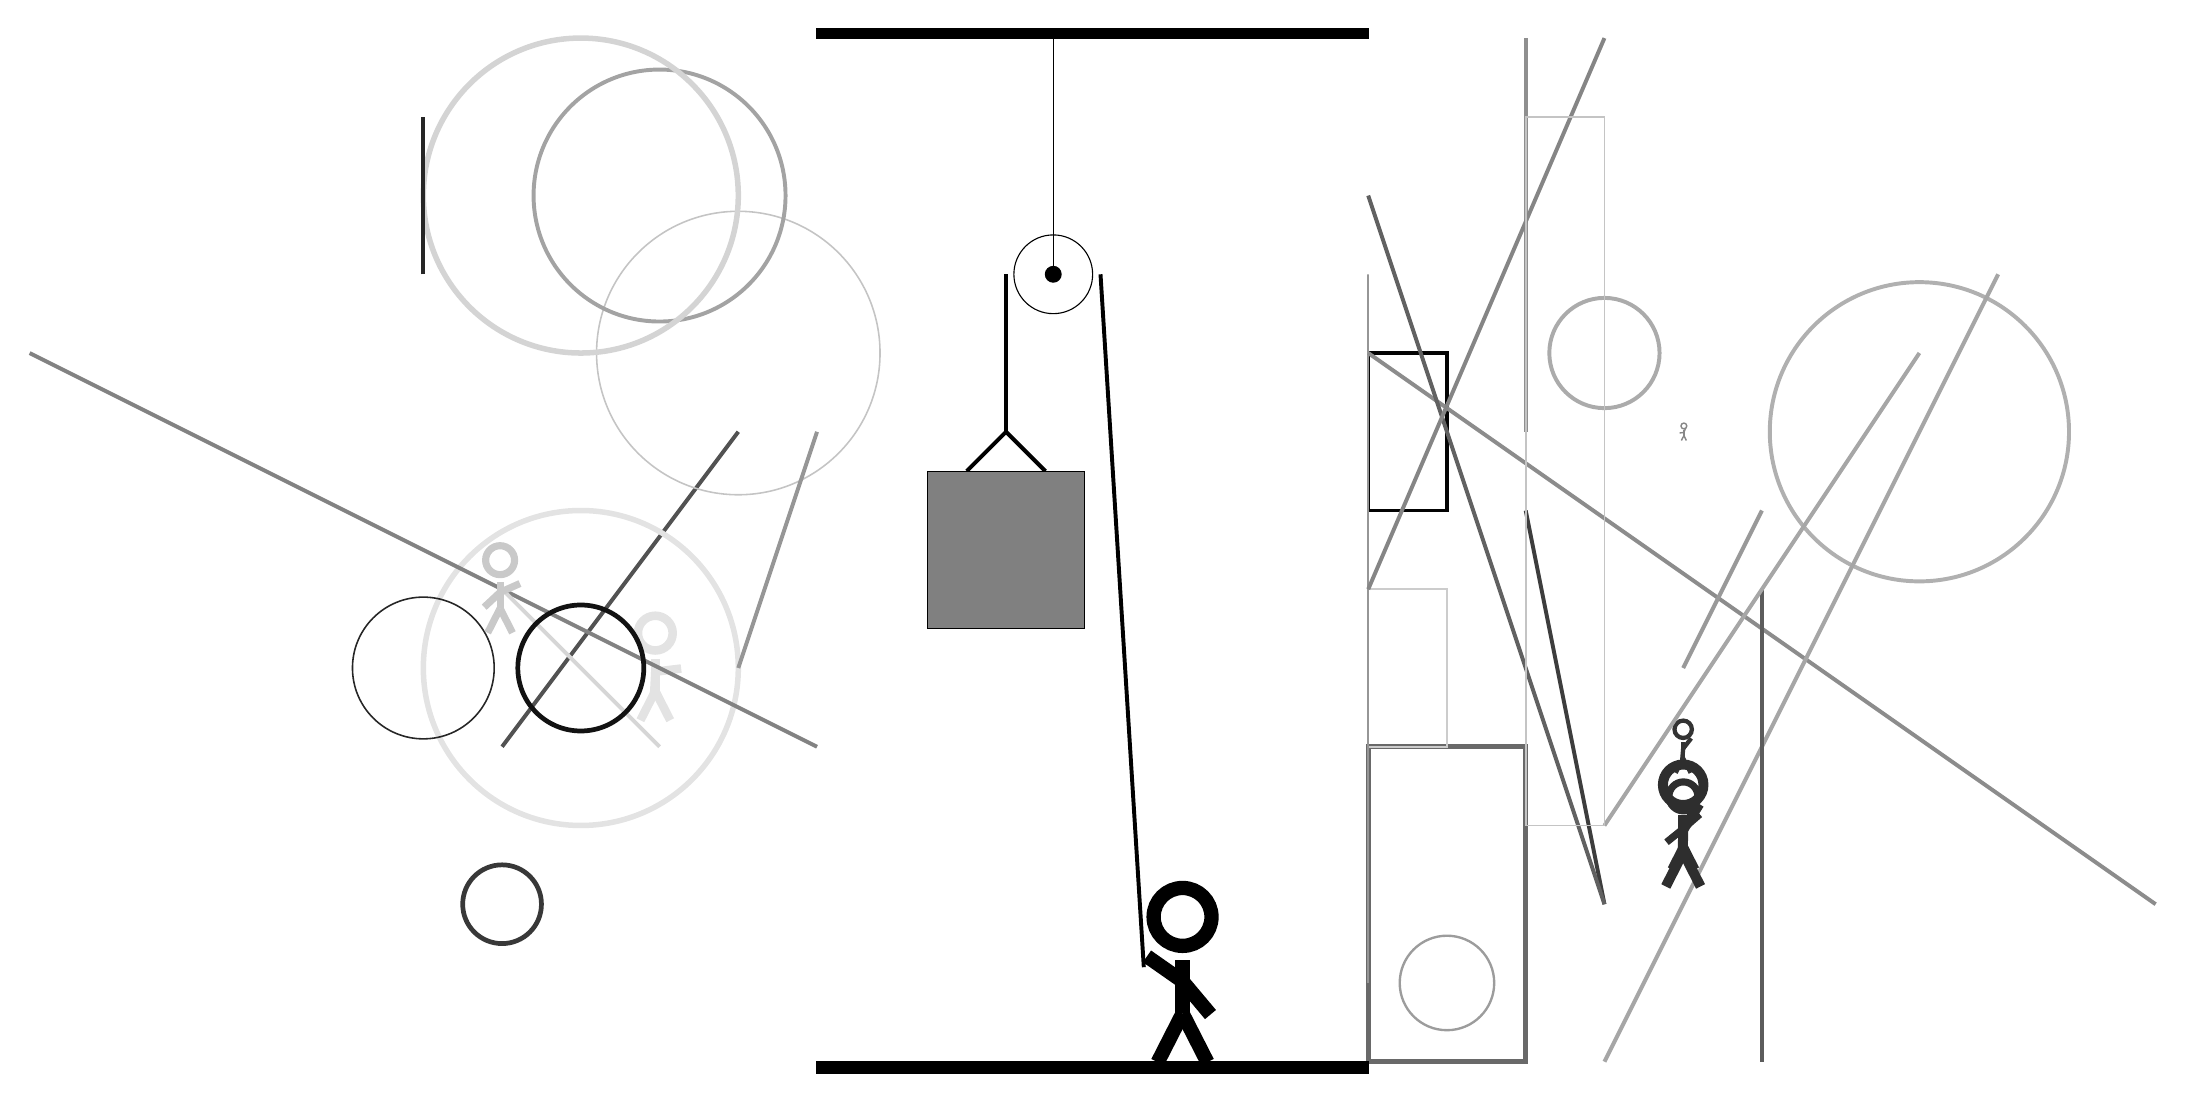
\begin{tikzpicture}
		%%%%% START %%%%%
		
		\draw[fill=black] (-2, 10) rectangle (5, 10.125);
		
		\draw (1, 7) circle (0.5);
		\draw[fill=black] (1, 7) circle (0.1);
		\draw (1, 10) -- (1, 7);
		
		\draw[line width=0.5mm] (-0.1, 4.5) -- (0.4, 5.0) -- (0.9, 4.5);
		\draw[fill=black!50] (-0.6, 4.5) rectangle (1.4, 2.5);
		
		\draw[line width=0.5mm] (0.4, 7) -- (0.4, 5.0);
		\centerarc[line width=0.5mm](1, 7)(0:180:0.6);
		\draw[line width=0.5mm](1.6, 7) -- (2.15, -1.8);
		
		\draw[line width=0.5mm, color=black!68](-3, 5) -- (-6, 1);
		
		\node[line width=0.2mm, color=black!82] at (9, 0) {\Strichmaxerl[5][39][41]};
		\draw[line width=0.6mm, color=black!59] (5, -3) rectangle (7, 1);
		\draw[line width=0.5mm, color=black!76](8, -1) -- (7, 4);
		\node[line width=0.4mm, color=black!11] at (-4, 2) {\Strichmaxerl[6][87][7]};
		\node[line width=0.4mm, color=black!80] at (9, 1) {\Strichmaxerl[3][85][52]};
		
		\draw [line width=0.7mm, color=black!11](-5, 2) circle (2.0);
		
		\draw[line width=0.2mm, color=black!20] (5, 1) rectangle (6, 3);
		\node[line width=0.4mm, color=black!47] at (9, 5) {\Strichmaxerl[1][8][68]};
		
		\draw[line width=0.4mm, color=black!99] (6, 6) rectangle (5, 4);
		
		\draw [line width=0.3mm, color=black!39](6, -2) circle (0.6);
		
		\draw [line width=0.2mm, color=black!85](-7, 2) circle (0.9);
		\draw[line width=0.5mm, color=black!44](7, 5) -- (7, 10);
		
		\draw[line width=0.3mm, color=black!41] (5, 7) rectangle (5, -2);
		\draw[line width=0.5mm, color=black!49](-2, 1) -- (-12, 6);
		\draw [line width=0.2mm, color=black!23](-3, 6) circle (1.8);
		
		\draw [line width=0.5mm, color=black!36](-4, 8) circle (1.6);
		
		\draw[line width=0.5mm, color=black!45](5, 6) -- (15, -1);
		\draw[line width=0.5mm, color=black!16](-4, 1) -- (-6, 3);
		
		\draw [line width=0.6mm, color=black!78](-6, -1) circle (0.5);
		\draw [line width=0.5mm, color=black!31](12, 5) circle (1.9);
		
		\draw[line width=0.5mm, color=black!62](8, -1) -- (5, 8);
		\draw [line width=0.7mm, color=black!17](-5, 8) circle (2.0);
		\node[line width=0.4mm, color=black!21] at (-6, 3) {\Strichmaxerl[5][43][24]};
		\draw[line width=0.5mm, color=black!41](-3, 2) -- (-2, 5);
		\draw [line width=0.5mm, color=black!33](8, 6) circle (0.7);
		\draw[line width=0.5mm, color=black!35](8, -3) -- (13, 7);
		\draw[line width=0.5mm, color=black!40](10, 4) -- (9, 2);
		\draw[line width=0.5mm, color=black!64](10, -3) -- (10, 3);
		
		\draw[line width=0.5mm, color=black!85](-7, 7) -- (-7, 9);
		\node[line width=0.3mm, color=black!82] at (9, 0) {\Strichmaxerl[7][89][58]};
		\draw [line width=0.6mm, color=black!93](-5, 2) circle (0.8);
		\draw[line width=0.5mm, color=black!48](8, 10) -- (5, 3);
		\draw[line width=0.5mm, color=black!35](8, 0) -- (12, 6);
		\draw[line width=0.2mm, color=black!23] (7, 0) rectangle (8, 9);
		
		\node at (2.6, -1.9) {\Strichmaxerl[10][-35][-50]};
		
		\draw[fill=black] (-2, -3) rectangle (5, -3.15);
		
		%%%%% END %%%%%
	\end{tikzpicture}
\end{document}